\documentclass[11pt,letterpaper]{article}
\usepackage[T1]{fontenc}
\usepackage{mathptmx}
\usepackage[margin=1in]{geometry}
\usepackage{amsmath,amssymb}
\usepackage{booktabs,tabularx}
\usepackage{enumitem}
\usepackage{tikz}
\usetikzlibrary{arrows.meta,positioning,fit,calc,backgrounds,shapes.geometric,decorations.pathreplacing}
\usepackage[font=small,labelfont=bf,textfont=it]{caption}
\usepackage{url}
\usepackage{xurl}
\emergencystretch=3em
\usepackage[hidelinks]{hyperref}
\usepackage{titlesec}
\titleformat{\section}{\normalfont\large\bfseries}{\thesection.}{0.5em}{}
\titleformat{\subsection}{\normalfont\normalsize\bfseries}{\thesubsection}{0.5em}{}
\setlength{\parindent}{1.5em}
\setlength{\parskip}{2pt}
\renewcommand{\arraystretch}{1.15}
\newcolumntype{Y}{>{\raggedright\arraybackslash}X}

\newcommand{\authorname}{Thor Thor}
\newcommand{\orcidid}{0009-0001-6573-385X}

\usepackage{amsthm}
\theoremstyle{plain}
\newtheorem{theorem}{Theorem}
\newtheorem{lemma}{Lemma}
\newtheorem{proposition}{Proposition}
\newtheorem{corollary}{Corollary}
\theoremstyle{definition}
\newtheorem{definition}{Definition}
\newtheorem{assumption}{Assumption}
\newtheorem{obligation}{Obligation}

% notation
\newcommand{\HR}{\mathsf{HighReach}}
\newcommand{\Reach}{\mathsf{Reach}}
\newcommand{\En}{\mathsf{Enabled}}
\newcommand{\SafeOpen}{\mathsf{SafeOpen}}
\newcommand{\Safe}{\mathsf{Safe}}
\newcommand{\Usable}{\mathsf{Usable}}
\newcommand{\Valid}{\mathsf{Valid}}
\newcommand{\Revoked}{\mathsf{Revoked}}
\newcommand{\Low}{\mathsf{Low}}
\newcommand{\Obs}{\mathsf{Obs}}
\newcommand{\KDF}{\mathsf{KDF}}
\newcommand{\Commit}{\mathsf{Commit}}
\newcommand{\Cg}{\mathcal{C}_g}
\newcommand{\Ca}{\mathcal{C}_a}
\newcommand{\Gs}{\mathcal{G}}
\newcommand{\enc}[1]{\langle #1\rangle}
\newcommand{\Rd}{\mathrel{\mathcal{R}_\delta}}

\tikzset{
  box/.style={draw, rectangle, rounded corners=1.5pt, align=center, font=\sffamily\scriptsize, minimum height=8mm, inner sep=3pt, fill=white},
  ebox/.style={draw, rectangle, dashed, align=center, font=\sffamily\scriptsize, minimum height=8mm, inner sep=3pt, fill=white},
  sbox/.style={draw, rectangle, rounded corners=1.5pt, align=center, font=\sffamily\scriptsize, minimum height=8mm, inner sep=3pt, fill=black!12},
  arr/.style={-{Stealth[length=2mm]}, semithick},
  darr/.style={-{Stealth[length=2mm]}, semithick, dashed},
  lbl/.style={font=\sffamily\tiny, fill=white, inner sep=1pt, align=center},
  capn/.style={font=\sffamily\scriptsize\itshape, align=center},
}

\hypersetup{pdftitle={Memory-Egress Cryptographic Interlock: A Hardware-Enforced Capability-Separation Model for AI Memory Security}, pdfauthor={Thor Thor}, pdfsubject={AI agent memory security, egress control, noninterference}, pdfkeywords={MECI; AI agents; memory security; egress control; confidential computing; noninterference; TLA+}}

\begin{document}

\begin{center}
{\LARGE\bfseries Memory-Egress Cryptographic Interlock: A Hardware-Enforced Capability-Separation Model for AI Memory Security\par}
\vspace{0.6em}
{\large Gated-Egress Safety, Epoch Non-Resurrection, and Noninterference Modulo Authorized Release\par}
\vspace{1.0em}
{\large \authorname\par}
\vspace{0.3em}
{\small Independent Open-Source Researcher, THOR-SEC\\
ORCID: \href{https://orcid.org/\orcidid}{\orcidid} \quad \url{codethor@gmail.com}\\
GitHub: \url{https://github.com/codethor0} \quad \url{https://codethor0.github.io/thor-sec/}\par}
\vspace{0.3em}
{\small This research was conducted independently on the author's own time and is not sponsored by, affiliated with, or representative of any employer.\par}
\vspace{0.3em}
{\small Preprint v1.0.0, October 2026. First shared publicly on 10 August 2026. Released openly for community review.\par}
\end{center}

\begin{abstract}
\noindent AI agents increasingly combine persistent memory with network, tool, file, and device capabilities. A compromised or manipulated agent can then hold readable protected state and a path through which that state can leave the trust boundary at the same time, and no instruction-level control removes that combination. This paper develops the Memory-Egress Cryptographic Interlock (MECI), a capability-separation pattern intended for hardware enforcement that makes unreleased protected information unreachable from every enabled gated egress channel. MECI formalizes high-to-egress reachability as reflexive-transitive closure over a state-dependent influence graph, gives an explicit labeling rule for sealed objects, defines a generation-checked, linearizable SafeOpen operation evaluated on the post-commit configuration, and separates gated egress from ambient observations such as timing, access patterns, and memory-bus traffic. We prove gated-egress safety from two local implementation obligations, show that a finite hazard projection refines the graph invariant under a stated soundness condition, prove epoch non-resurrection, give a counterexample showing that memory-egress mutual exclusion does not imply noninterference, and prove noninterference modulo an explicit authorized-release function in which the MECI invariant, rather than an assumed output property, carries the gated-output step. The finite safety core is specified in TLA+ and checked exhaustively within stated bounds by TLC and by an independent dependency-free reference checker. The two agree exactly on reachable-state counts for all five modeled designs, find no violation in the atomic and generation-checked designs, and return shortest counterexamples for three deliberately weakened designs. The paper also gives an Arm CCA/RMM refinement path, a GPU quiescence contract, a representative declassification policy for an AI incident-triage agent, and a comparison with CHERI, seL4, and WASI. No current confidential-computing platform is claimed to implement MECI; the work is a formal specification and falsifiable research program.
\end{abstract}
\vspace{-0.4em}
\noindent\textbf{Keywords:} AI agents; memory security; egress control; confidential computing; noninterference; declassification; capability security; trusted execution environments; formal methods; TLA+
\medskip

\noindent\textbf{Open-source research statement.} This is independent open-source research derived from publicly accessible vendor documentation, published or openly available research, and reproducible formal artifacts developed for this paper. The model, reference checker, captured outputs, and TLA+ specification are released with the paper. The abstract theorems are proved under stated assumptions; platform-level guarantees require refinement and implementation evidence. No claim of peer review, production deployment, or measured end-to-end hardware performance is made.

\section{Introduction}

AI agents are moving from stateless text generation toward systems that remember prior interactions, retrieve user-specific context, invoke third-party tools, execute code, and communicate with external services. The resulting attack surface differs qualitatively from that of a conventional application. Memory and authority are assembled dynamically inside a planner loop, while the same process may call browsers, APIs, databases, file systems, or Model Context Protocol (MCP) servers. Recent formal work on agentic information flow treats the planner and tool loop as a security boundary that requires explicit semantics rather than prompt-level trust \cite{llmbda}, and recent MCP studies show that tool metadata alone can steer an agent toward high-privilege tools \cite{mcpitp,mcpshield}.

The MECI proposal starts from a deliberately simple question: should a machine ever allow protected memory to be readable while an externally observable egress capability is simultaneously available? In its first form, external egress was represented by $E_t$, protected-memory decryptability by $D_t$, and readable secret-dependent plaintext by $P_t$. The invariant was
\begin{equation}\label{eq:orig}
\Phi_t = \neg\big(E_t \wedge (D_t \vee P_t)\big),
\end{equation}
or equivalently $E_t = 1 \Rightarrow D_t = P_t = 0$. The intended transition order was to revoke decryption, purge secret-dependent plaintext, and only then enable egress.

That formulation captures an important design instinct, but it is not a sufficient security theorem for a real AI system. It treats decryption as a single bit, ignores secret-derived buffers and microarchitectural state, conflates all observations with the network interface, and assumes that deleting readable state makes future output independent of a prior secret. This paper keeps the capability-separation idea and tightens the claim to what can be proved and checked.

\subsection{Contributions}
\begin{enumerate}[leftmargin=*,itemsep=1pt]
\item A state-dependent \emph{influence-graph reachability invariant} over gated egress channels and unreleased protected objects, using reflexive-transitive closure, with an explicit labeling rule for sealed (encrypted-at-rest) objects.
\item A separation of \emph{gated channels}, which a reference monitor can disable, from \emph{ambient observation channels}, which require separate noninterference, microarchitectural, cryptographic, or physical assumptions.
\item A generation-checked SafeOpen control block whose final check is evaluated on the post-commit configuration at an explicit linearization point, and a proof of the stale-snapshot failure that occurs without generation validation.
\item Proofs of gated-egress safety from two local obligations, of refinement from a finite hazard projection to the graph invariant, and of epoch non-resurrection, followed by a counterexample showing that these safety results alone do not imply noninterference.
\item An explicit release function for a representative AI incident-triage agent and a conditional noninterference theorem in which a low-determinism lemma derived from the MECI invariant carries the gated-output step.
\item A TLA+ specification of the finite safety core, checked by TLC and by an independent reference checker that agree exactly on reachable-state counts, with negative controls for stale permits, incomplete guards, export-buffer leakage, release-policy widening, and epoch rollback.
\item A concrete Arm CCA/RMM refinement path and a GPU quiescence contract that distinguish present vendor guarantees from proposed MECI mechanisms.
\item A comparison with CHERI, seL4, and WASI, and a statement of MECI's relation to the author's prior work on epoch isolation (MIAM) and influence-versus-authority reasoning (ACN).
\end{enumerate}

Section~\ref{sec:related} positions MECI against prior work. Sections~\ref{sec:threat}--\ref{sec:epoch} define the threat model, the formal model, and the epoch interlock. Section~\ref{sec:safety} proves the safety results and Section~\ref{sec:ni} the conditional noninterference theorem. Section~\ref{sec:check} reports model checking. Sections~\ref{sec:ambient}--\ref{sec:failure} cover ambient channels, platform refinement, architecture, agent memory semantics, performance, and failure handling. Sections~\ref{sec:obligations}--\ref{sec:release} list open obligations, limitations, and the release boundary.

\section{Research Position and Relation to Prior Work}\label{sec:related}

\textbf{Information-flow security.} Noninterference states end-to-end confidentiality as indistinguishability of low observations across runs that differ only in high inputs \cite{goguen1982,sabelfeld2003}. Useful systems release some secret-dependent information, so controlled declassification is a separate mechanism with its own theory \cite{myers2006,arden2021}. The LLMbda calculus gives agent planner loops, tool calls, and LLM conversations an information-flow semantics with a noninterference theorem \cite{llmbda}. MECI claims no novelty in declassification theory. Its contribution is a hardware-oriented enforcement boundary that constrains \emph{when} unreleased high state may coexist with egress authority.

\textbf{Capability systems.} CHERI adds unforgeable, tagged capabilities with bounds, permissions, provenance, and monotonic restriction to general-purpose ISAs \cite{cheri}. seL4 combines capability-based resource control with machine-checked functional correctness and information-flow proofs for supported configurations \cite{murray2013,sel4docs}. WASI grants host resources through link-time imports and unforgeable runtime handles \cite{wasi}. Table~\ref{tab:cap} summarizes how each relates to MECI. These systems can supply the concrete authority graph from which $\Reach_s$ is computed; MECI adds a temporal cross-domain rule bound to cryptographic epochs and explicit release.

\begin{table}[t]
\centering\small
\caption{MECI compared with established capability-security substrates.}\label{tab:cap}
\begin{tabularx}{\textwidth}{@{}p{1.3cm}YYY@{}}
\toprule
System & Core capability property & Contribution to MECI & Distinction from MECI\\
\midrule
CHERI & Unforgeable tagged capabilities with bounds, permissions, provenance, and monotonic restriction in the ISA \cite{cheri}. & Makes memory and object authority, and some reachability edges, concrete and hardware-enforced. & No epoch-bound temporal rule that egress authority and unreleased high reachability are mutually exclusive.\\
seL4 & Capability-based microkernel with machine-checked functional and information-flow proofs for supported configurations \cite{murray2013,sel4docs}. & Strong reference-monitor substrate and precedent for proving confidentiality over a capability graph. & MECI adds a cryptographic epoch lifecycle and a cross-device SafeOpen cut; device and IOMMU assumptions remain configuration-specific.\\
WASI & Link-time imports and unforgeable runtime handles grant access to host resources \cite{wasi}. & Application and tool layer for expressing which resources and egress services a component may hold. & Runtime capability confinement is not hardware memory confidentiality or a non-resurrectable machine epoch.\\
MECI & State-dependent high-to-egress reachability prohibition plus SafeOpen and epoch revocation. & Composes with the systems above. & Targets the transition between protected computation and externally observable authority.\\
\bottomrule
\end{tabularx}
\end{table}

\textbf{Hardware information flow.} SecVerilog and later hardware information-flow work show that timing-sensitive noninterference can be expressed and verified at the hardware-design level \cite{secverilog,cheang2023}. In a MECI refinement, such tools can verify that RTL or microarchitectural transitions preserve the labels and observational equivalence that the abstract graph assumes.

\textbf{Confidential computing and its side channels.} Arm CCA with Memory Encryption Contexts, Intel TDX, AMD SEV-SNP, and NVIDIA confidential computing provide isolation, attestation, and memory or device protection in different combinations \cite{armmec,inteltdx,amdsnp,nvidiablog}. They are enabling substrates, not substitutes for the temporal reachability invariant. CipherSteal recovers neural-network inputs from ciphertext write behavior of TEE-shielded execution \cite{ciphersteal}; TEE.fail breaks Intel and AMD confidential-computing guarantees through DDR5 memory-bus interposition \cite{teefail}; TDXRay builds cache-line-granular host-side access traces of unmodified Intel TDX guests from four new side-channel primitives \cite{tdxray}; a recent survey catalogs memory side-channel classes more broadly \cite{hassan2025}. These results motivate MECI's explicit ambient-channel partition rather than any claim that egress gating closes all observation channels.

\textbf{Relation to the author's prior work.} Mission-Invariant Architecture Morphing (MIAM) binds service authority to cryptographic epochs that are retired when the service graph changes \cite{miam}. MECI applies the same epoch discipline to the memory-egress boundary and adopts MIAM's injective tuple encoding for key-derivation inputs (Section~\ref{sec:epoch}). Attack Calculus (ACN) separates influence over an AI agent from the authority the agent holds and checks authority with a capability order \cite{acn}. The rogue-agent walkthrough in Section~\ref{sec:rogue} is an instance of that separation: a planner that an attacker fully influences still lacks the authority to change labels, widen the release policy, or commit the egress mask.

\section{Threat Model and Security Objective}\label{sec:threat}

\subsection{Adversary}
The modeled adversary may control or manipulate agent-level software behavior, including prompts, tool descriptions, retrieved content, planner decisions, and tool-call parameters, and may induce arbitrary sequences of allowed software operations. In stronger deployment profiles, the host operating system or hypervisor may also be untrusted, subject to the guarantees of the selected confidential-computing platform.

The adversary is assumed not to break the underlying cryptographic primitives. Whether physical access, supply-chain compromise, power analysis, electromagnetic observation, or memory-bus interposition is in scope is a separate profile decision. This matters because modern TEEs intentionally exclude some physical attacks. TEE.fail demonstrates practical DDR5 interposition against Intel TDX and AMD SEV-SNP \cite{teefail}, and both vendors responded that such physical attacks are outside the published threat models of the affected TEEs \cite{intelteefail,amdsb3040}.

\subsection{Two channel classes}
Let $\mathcal{C}$ be the set of attacker-observable channels. We partition it as
\begin{equation}
\mathcal{C} = \Cg \cup \Ca,
\end{equation}
where $\Cg$ is the set of \emph{gated channels} and $\Ca$ the set of \emph{ambient channels}. Typical members of $\Cg$ include network transmit paths, MCP or other tool invocations, file writes that cross the trust boundary, clipboard and IPC paths, device output queues, and explicit export APIs. A reference monitor can mediate these.

Typical members of $\Ca$ include cache timing, secret-dependent memory access patterns, encrypted-memory write patterns visible to a malicious host, shared-resource contention, physical bus observations, power, electromagnetic radiation, and acoustic leakage. Ambient observations made \emph{during} protected computation cannot be repaired by purging memory afterward; CipherSteal and TDXRay demonstrate this class directly \cite{ciphersteal,tdxray}.

\begin{figure}[t]
\centering
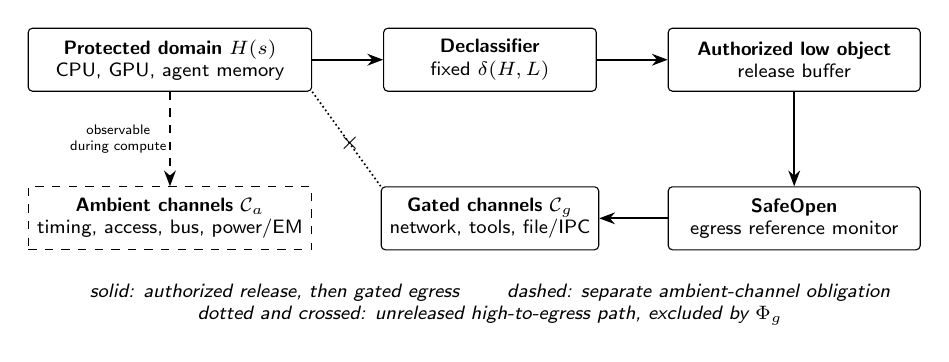
\begin{tikzpicture}[node distance=7mm and 9mm]
\node[box, minimum width=36mm] (pd) {\textbf{Protected domain} $H(s)$\\CPU, GPU, agent memory};
\node[box, right=of pd, minimum width=27mm] (dec) {\textbf{Declassifier}\\fixed $\delta(H,L)$};
\node[box, right=of dec, minimum width=32mm] (rel) {\textbf{Authorized low object}\\release buffer};
\node[box, below=12mm of rel, minimum width=32mm] (so) {\textbf{SafeOpen}\\egress reference monitor};
\node[box, below=12mm of dec, minimum width=27mm] (gc) {\textbf{Gated channels} $\Cg$\\network, tools, file/IPC};
\node[ebox, below=12mm of pd, minimum width=36mm] (amb) {\textbf{Ambient channels} $\Ca$\\timing, access, bus, power/EM};
\draw[arr] (pd) -- (dec);
\draw[arr] (dec) -- (rel);
\draw[arr] (rel) -- (so);
\draw[arr] (so) -- (gc);
\draw[darr] (pd) -- node[lbl, left]{observable\\during compute} (amb);
\draw[semithick, densely dotted] (pd.south east) -- node[pos=0.55, font=\sffamily\small]{$\times$} (gc.north west);
\node[capn, below=3mm of gc] {solid: authorized release, then gated egress \qquad dashed: separate ambient-channel obligation\\dotted and crossed: unreleased high-to-egress path, excluded by $\Phi_g$};
\end{tikzpicture}
\caption{Capability-cut view of MECI. Protected information may reach gated egress only through an authorized declassifier and the SafeOpen reference monitor. Ambient observations are a separate security obligation because they can occur during protected computation.}
\label{fig:cut}
\end{figure}

\section{Formal Model}\label{sec:model}

\subsection{Objects, influence graph, and reachability}
Let $S$ be the set of machine states. For each $s \in S$, define a directed, state-dependent influence graph
\begin{equation}
\Gs_s = (V_s, A_s, \ell_s),
\end{equation}
where $V_s$ contains information-bearing objects, active authorities, declassifier nodes, and attacker-observable channel endpoints; $A_s \subseteq V_s \times V_s$ is the direct influence relation; and $\ell_s : V_s \to \{H, L, D\}$ labels each vertex high, low, or authorized declassifier.

A direct edge $x \to_s y$ exists exactly when the active configuration permits information in $x$ to affect $y$ without an intervening security decision. The relation covers explicit and implicit dependencies at the model boundary: loads and stores, aliases, shared buffers, queue descriptors, DMA mappings, device command streams, tool-call argument construction, capability delegation, control decisions whose outcome is externally visible, and scheduler or timing edges when those observations are in the deployment profile. A platform refinement is sound only if every concrete information path in the deployment threat model induces a corresponding edge.

Let $A^{\delta}_s \subseteq A_s$ be the set of edges \emph{leaving} a $D$-labeled vertex whose carried value is exactly a value permitted by the release function $\delta$ (Section~\ref{sec:release-fn}). Edges into a declassifier remain in the graph, so a declassifier with any unauthorized output still connects its high inputs to that output. Define the unreleased graph $\Gs^{-\delta}_s = (V_s, A_s \setminus A^{\delta}_s, \ell_s)$ and, for $x, y \in V_s$,
\begin{equation}\label{eq:reach}
\Reach_s(x,y) \equiv (x,y) \in (A_s \setminus A^{\delta}_s)^{*},
\end{equation}
where $(\cdot)^{*}$ is reflexive-transitive closure. For a gated channel $c$ with endpoint $v_c \in V_s$,
\begin{equation}\label{eq:highreach}
\HR(c,s) \equiv \exists x \in V_s : \ell_s(x) = H \wedge \Reach_s(x, v_c).
\end{equation}
Reflexivity matters: if the endpoint itself holds high data (for example, a send buffer into which a secret was copied), $\HR$ must be true even when no edge enters the endpoint. A transitive-only closure misses this case (Section~\ref{sec:check}, graph checks). Let $\En(c,s)$ mean that the endpoint can currently produce an attacker-observable effect, and write $E(s) \equiv \exists c \in \Cg : \En(c,s)$.

\begin{definition}[Gated-egress invariant]\label{def:phig}
\[
\boxed{\;\Phi_g(s) \equiv \forall c \in \Cg : \En(c,s) \Rightarrow \neg\HR(c,s).\;}
\]
\end{definition}

This definition makes the implementation burden explicit. A newly discovered tool, alias, DMA mapping, derived buffer, or control dependency is not handled by adding prose; it must appear as a vertex or edge in $\Gs_s$. Conversely, a value that has passed through a confined declassifier leaves on an authorized edge in $A^{\delta}_s$ and can become low without declaring all secret-dependent state illegal.

\subsection{Sealed objects}
MECI keeps protected state sealed at rest while egress is open; otherwise every egress interval would require destroying all protected memory. The graph therefore needs a rule for ciphertext. If ciphertext were always high, $\Phi_g$ could not hold whenever a storage-backed tool can reach sealed state; if it were always low, a usable key would silently reconnect it to plaintext.

\begin{assumption}[Sealed-object confidentiality]\label{as:aead}
Sealing uses an authenticated-encryption scheme with associated data \cite{rogaway2002} that provides ciphertext indistinguishability and integrity under the deployment's key-use limits, with nonces that never repeat under a key and ciphertext lengths padded to policy-defined size classes.
\end{assumption}

\begin{definition}[Sealed-object labeling]\label{def:seal}
A vertex holding an object sealed under a domain key $K^{d}_{e}$ is labeled $L$ in $\Gs_s$ if no key able to open it is usable in $s$ (Section~\ref{sec:epoch}) and its size class is part of the authorized release; otherwise it is labeled $H$.
\end{definition}

Deterministic memory encryption inside a TEE is not sealing in this sense. Its ciphertext is observable while the key is live, so those observations belong to $\Ca$ (Section~\ref{sec:ambient}).

\subsection{Strict finite projection}
For model checking and implementation profiles, a finite Boolean projection is useful. Let
\begin{center}
\begin{tabular}{@{}ll@{}}
$D$: & the current-epoch decryption capability $\tau_{e}$ is not yet revoked, \\
$P$: & readable protected plaintext remains architecturally resident, \\
$M$: & secret-dependent microarchitectural residue remains, \\
$I$: & a DMA-capable path can reach protected memory, \\
$G$: & secret-dependent accelerator or device state remains, \\
$B$: & an unreleased high object exists in an exportable buffer, \\
$Q$: & a high-producing execution unit can still create high state.
\end{tabular}
\end{center}
The strict finite invariant is
\begin{equation}\label{eq:phibit}
\Phi_{bit}(s) = \neg\big(E \wedge (D \vee P \vee M \vee I \vee G \vee B \vee Q)\big).
\end{equation}
$B$ closes the ``copy the secret, purge memory, then send the copy'' counterexample (Proposition~\ref{prop:export}). $Q$ prevents a racing core, accelerator, or DMA producer from recreating high state between cleanup and egress enable. The projection is useful only if clearing the bits really removes high reachability, which we state as an obligation on the implementation profile.

\begin{assumption}[Projection soundness]\label{as:proj}
For every reachable $s$: if $\neg(D \vee P \vee M \vee I \vee G \vee B \vee Q)$ holds in $s$, then $\forall c \in \Cg : \neg\HR(c,s)$.
\end{assumption}

\subsection{Safety predicate and linearizable SafeOpen}
Define
\begin{equation}\label{eq:safe}
\Safe(s) \equiv \neg D \wedge \neg P \wedge \neg M \wedge \neg I \wedge \neg G \wedge \neg B \wedge \neg Q \wedge \mathit{FreshEpoch}(s).
\end{equation}
The only operation that may change a gated channel from disabled to enabled is SafeOpen. For a requested channel set $R \subseteq \Cg$, let $\Commit_R(s)$ be the configuration that equals $s$ except that the egress mask is $R$. The final check is evaluated on that post-commit configuration:
\begin{align}
\SafeOpen(s, s', R) \Rightarrow{}& E(s) = 0 \wedge \Safe(s) \wedge s' = \Commit_R(s) \label{eq:so1}\\
&\wedge \forall c \in R : \neg\HR(c, s') \wedge E_R(s') = 1. \label{eq:so2}
\end{align}
Enabling a channel can itself activate edges, for example by mapping a buffer into a NIC descriptor ring. Because $\Commit_R$ changes only the egress mask, the monitor can compute $\Gs_{s'}$ from $\Gs_s$ and $R$ before committing, so evaluating the check on $s'$ is implementable.

\textbf{MECI Control Block.} A concrete design uses a small trusted MECI Control Block (MCB) below the hostile OS and agent boundary. The MCB owns the hardware-visible egress mask and stores at least
\begin{equation}
\langle \mathit{epoch}, \mathit{gen}, \mathit{complete}, \mathit{egressMask}, \mathit{policyHash}, \mathit{releaseDigest}\rangle.
\end{equation}
Every trusted-state mutation that can falsify $\Safe$ or make $\HR$ true increments $\mathit{gen}$. Domain cleanup sets bits in $\mathit{complete}$ only for the current generation. The MCB exposes four primitives:
\begin{enumerate}[leftmargin=*,itemsep=1pt]
\item $\mathsf{Freeze}(e)$: disable new high-producing work and return the current generation $g$.
\item $\mathsf{MarkDone}(d,e,g)$: record completion for a required domain $d$ only if $e$ and $g$ are still current.
\item $\SafeOpen(R,e,g,r)$: recompute the final safety predicate and $\HR$ on $\Commit_R(s)$, require the expected epoch and generation, verify the required completion bits and the release digest $r$, then commit the egress mask.
\item $\mathsf{Close}()$: clear the egress mask before any protected capability can be issued for a new epoch.
\end{enumerate}
The linearization point is the trusted commit that changes $\mathit{egressMask}$ from zero to $R$ after the final validation. A check performed earlier in software is not the linearization point. If any high-producing state changes after a preparatory check, $\mathit{gen}$ changes and the stale permit cannot commit. Failure, timeout, reset, or crash before the commit leaves $\mathit{egressMask} = 0$.

\begin{figure}[t]
\centering
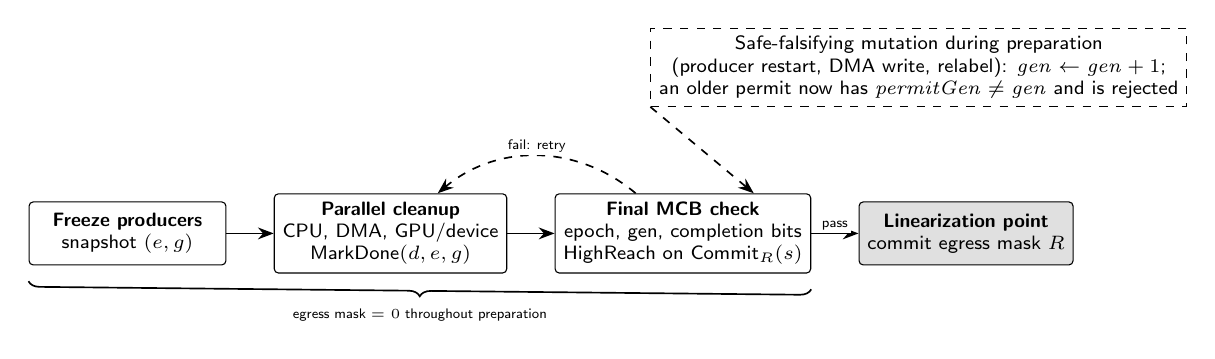
\begin{tikzpicture}[node distance=6mm]
\node[box, minimum width=25mm] (fr) {\textbf{Freeze producers}\\snapshot $(e,g)$};
\node[box, right=of fr, minimum width=27mm] (cl) {\textbf{Parallel cleanup}\\CPU, DMA, GPU/device\\$\mathsf{MarkDone}(d,e,g)$};
\node[box, right=of cl, minimum width=30mm] (ck) {\textbf{Final MCB check}\\epoch, gen, completion bits\\$\HR$ on $\Commit_R(s)$};
\node[sbox, right=of ck, minimum width=26mm] (lp) {\textbf{Linearization point}\\commit egress mask $R$};
\draw[arr] (fr) -- (cl);
\draw[arr] (cl) -- (ck);
\draw[arr] (ck) -- node[lbl, above]{pass} (lp);
\draw[darr] ([xshift=-6mm]ck.north) to[out=140, in=40] node[lbl, above]{fail: retry} ([xshift=6mm]cl.north);
\node[ebox, above=12mm of lp, xshift=-6mm, minimum width=56mm] (mut) {Safe-falsifying mutation during preparation\\(producer restart, DMA write, relabel): $\mathit{gen} \leftarrow \mathit{gen}+1$;\\an older permit now has $\mathit{permitGen} \neq \mathit{gen}$ and is rejected};
\draw[darr] (mut.south west) -- ([xshift=9mm]ck.north);
\draw[decorate, decoration={brace, amplitude=4pt, mirror}, semithick] ([yshift=-2mm]fr.south west) -- ([yshift=-2mm]ck.south east) node[midway, below=5pt, font=\sffamily\tiny]{egress mask $=0$ throughout preparation};
\end{tikzpicture}
\caption{Concrete SafeOpen transaction. Cleanup may be multi-step and concurrent, but the final check and the egress-mask commit must be one linearized step of the trusted monitor. A generation counter invalidates stale safety snapshots.}
\label{fig:safeopen}
\end{figure}

\begin{proposition}[Stale-snapshot failure]\label{prop:stale}
If a system evaluates $\Safe(s)$, records an unversioned permit, later allows a protected producer to restart, and then enables egress using only that permit, the gated-egress invariant can be violated even though the earlier check was correct.
\end{proposition}
\begin{proof}
Reach a state with all hazards cleared and evaluate $\Safe = \mathit{true}$. Before egress commits, restart a producer so $Q := 1$. If this mutation does not invalidate the permit, the split open step sets $E := 1$ while $Q = 1$, so $\Phi_{bit}$ is false. A generation-checked permit prevents the final step because $\mathit{permitGen} \neq \mathit{gen}$ after the restart. Both TLC and the reference checker return this trace as the shortest counterexample for the unversioned design (Section~\ref{sec:check}).
\end{proof}

\subsection{Lifecycle}
Figure~\ref{fig:life} shows the lifecycle. Egress is open in exactly one state, EXTERNAL. Every other state, including failure paths, keeps the egress mask at zero. A useful forward partial order is
\begin{equation}
\mathit{Freeze} \prec \mathit{Quiesce} \prec \mathit{VerifySafe} \prec E{\uparrow},
\end{equation}
with revocation, DMA quarantine, memory cleanup, and device cleanup complete before $\mathit{VerifySafe}$ succeeds. Their internal order can vary if no step can reopen egress and no producer can recreate high state.

\begin{figure}[t]
\centering
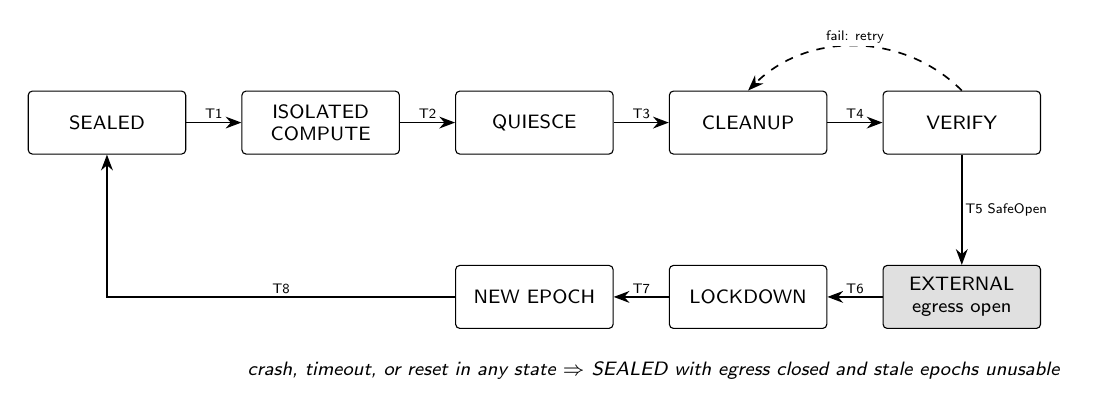
\begin{tikzpicture}[node distance=7mm]
\node[box, minimum width=20mm] (sea) {SEALED};
\node[box, right=of sea, minimum width=20mm] (iso) {ISOLATED\\COMPUTE};
\node[box, right=of iso, minimum width=20mm] (qui) {QUIESCE};
\node[box, right=of qui, minimum width=20mm] (cle) {CLEANUP};
\node[box, right=of cle, minimum width=20mm] (ver) {VERIFY};
\node[sbox, below=14mm of ver, minimum width=20mm] (ext) {EXTERNAL\\egress open};
\node[box, left=of ext, minimum width=20mm] (loc) {LOCKDOWN};
\node[box, left=of loc, minimum width=20mm] (new) {NEW EPOCH};
\draw[arr] (sea) -- node[lbl, above]{T1} (iso);
\draw[arr] (iso) -- node[lbl, above]{T2} (qui);
\draw[arr] (qui) -- node[lbl, above]{T3} (cle);
\draw[arr] (cle) -- node[lbl, above]{T4} (ver);
\draw[arr] (ver) -- node[lbl, right]{T5 SafeOpen} (ext);
\draw[arr] (ext) -- node[lbl, above]{T6} (loc);
\draw[arr] (loc) -- node[lbl, above]{T7} (new);
\draw[arr] (new) -| node[lbl, pos=0.25, above]{T8} (sea);
\draw[darr] (ver.north) to[out=135, in=45] node[lbl, above]{fail: retry} (cle.north);
\node[capn, below=3mm of loc, xshift=-12mm] (fc) {crash, timeout, or reset in any state $\Rightarrow$ SEALED with egress closed and stale epochs unusable};
\end{tikzpicture}
\\[2mm]
{\sffamily\tiny T1 attest/derive \quad T2 freeze producers \quad T3 quiesce \quad T4 cleanup done \quad T5 SafeOpen \quad T6 close egress \quad T7 verify/advance epoch \quad T8 issue fresh epoch capability}
\caption{MECI lifecycle. EXTERNAL (shaded) is the only state with egress open. Cleanup and verification may retry while egress stays closed; failures return to SEALED. The security-critical linearization point is T5.}
\label{fig:life}
\end{figure}

\section{Cryptographic Epoch Interlock}\label{sec:epoch}

Let $K_R$ be a root secret held by a hardware root of trust or key-management service, $e \in \mathbb{N}$ the isolation epoch, $c$ a monotonic anti-rollback counter, $\tau_e$ a non-exportable epoch capability, $\sigma_e$ a per-epoch seed held inside the key service, $d$ a domain separator, $\pi_e$ a canonical policy description, and $A_e$ an attested configuration measurement. Domain keys are derived as
\begin{equation}\label{eq:kdf}
K^{d}_{e} = \KDF\big(K_R,\ \enc{\texttt{"MECI-v1"},\, e,\, c,\, \sigma_e,\, d,\, H(\pi_e),\, H(A_e)}\big).
\end{equation}
Here $\enc{\cdot}$ is the injective tuple encoding used in MIAM \cite{miam}: each field carries a fixed-width type tag and a 32-bit big-endian length followed by its bytes, and the number of fields is fixed per context label. Raw concatenation is never used, so no two distinct input tuples share an encoding. The capability $\tau_e$ is not itself a KDF input; it gates whether the key service will evaluate Equation~\eqref{eq:kdf} for epoch $e$ at all. The policy and attestation bindings prevent a valid epoch from being replayed under a different egress policy, software measurement, or device configuration.

\begin{figure}[t]
\centering
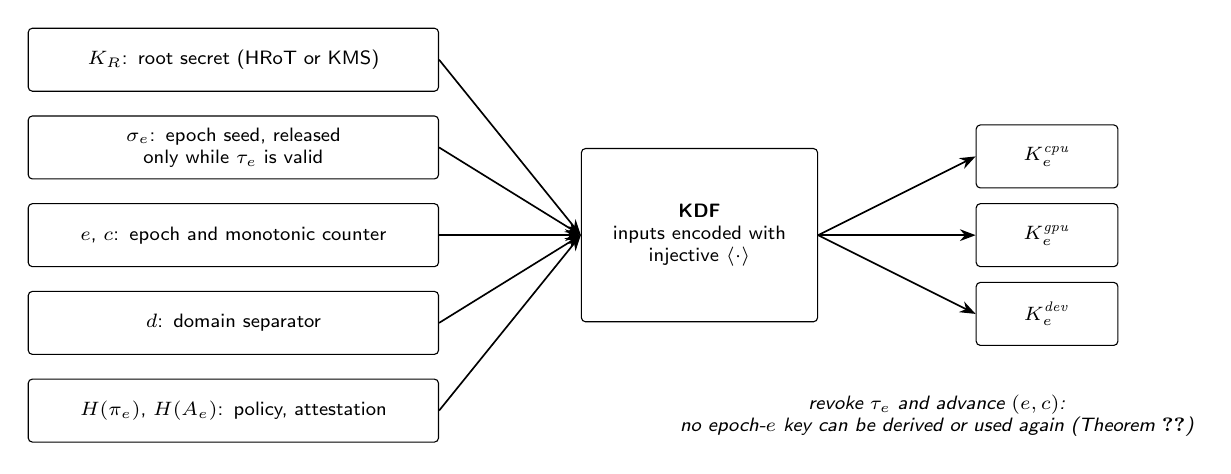
\begin{tikzpicture}[node distance=3mm]
\node[box, text width=50mm] (kr) {$K_R$: root secret (HRoT or KMS)};
\node[box, below=of kr, text width=50mm] (se) {$\sigma_e$: epoch seed, released only while $\tau_e$ is valid};
\node[box, below=of se, text width=50mm] (ec) {$e$, $c$: epoch and monotonic counter};
\node[box, below=of ec, text width=50mm] (dd) {$d$: domain separator};
\node[box, below=of dd, text width=50mm] (pa) {$H(\pi_e)$, $H(A_e)$: policy, attestation};
\node[box, right=18mm of ec, minimum width=30mm, minimum height=22mm] (kdf) {\textbf{KDF}\\inputs encoded with\\injective $\enc{\cdot}$};
\node[box, right=20mm of kdf, yshift=10mm, minimum width=18mm] (k1) {$K^{\mathit{cpu}}_{e}$};
\node[box, right=20mm of kdf, minimum width=18mm] (k2) {$K^{\mathit{gpu}}_{e}$};
\node[box, right=20mm of kdf, yshift=-10mm, minimum width=18mm] (k3) {$K^{\mathit{dev}}_{e}$};
\foreach \n in {kr,se,ec,dd,pa} \draw[arr] (\n.east) -- (kdf.west);
\foreach \n in {k1,k2,k3} \draw[arr] (kdf.east) -- (\n.west);
\node[capn, below=5mm of k3, xshift=-14mm] {revoke $\tau_e$ and advance $(e,c)$:\\no epoch-$e$ key can be derived or used again (Theorem~\ref{thm:epoch})};
\end{tikzpicture}
\caption{Epoch and domain key separation. All inputs enter the KDF in parallel through an injective encoding. The construction is abstract; no current TEE is claimed to expose these exact key controls.}
\label{fig:kdf}
\end{figure}

Key use is governed by the rule
\begin{equation}\label{eq:keyuse}
\Usable(K^{d}_{e}, s) \Rightarrow \Valid(\tau_e, s) \wedge e = \mathit{CurrentEpoch}(s) \wedge c = \mathit{Counter}(s),
\end{equation}
and the projection bit $D$ holds exactly when $\neg\Revoked(\tau_{\mathit{CurrentEpoch}(s)}, s)$. This is how the TLA+ model in Section~\ref{sec:check} derives $D$.

\begin{assumption}[Irreversible revocation]\label{as:revoke}
$\Revoked(\tau_e) \Rightarrow \Box\neg\Valid(\tau_e)$.
\end{assumption}

\begin{assumption}[Monotonic epoch]\label{as:mono}
The persistent epoch and counter state, held in rollback-protected storage, never decreases: $e_{t+1} \ge e_t$ and $c_{t+1} \ge c_t$.
\end{assumption}

\section{Safety Results}\label{sec:safety}

The safety theorem rests on two local obligations. Neither is a lemma about source code; each is a property the trusted implementation must establish.

\begin{obligation}[Local egress guard]\label{ob:guard}
For every transition $s \to s'$ and channel $c$ with $\neg\En(c,s) \wedge \En(c,s')$: $\Safe(s)$ holds, $\neg\HR(c,s')$ holds, and the check and the commit form one linearized step of the trusted monitor, so no transition that can falsify $\Safe$ is linearized between them.
\end{obligation}

A software check followed by an independently writable NIC register does not satisfy Obligation~\ref{ob:guard} under a hostile kernel. The check and enable must be mediated by the trusted reference monitor, firmware, hypervisor extension, device security controller, or an equivalent trusted component.

\begin{obligation}[Reachability creation]\label{ob:create}
For every transition $s \to s'$ and channel $c \in \Cg$: $\neg\HR(c,s) \wedge \HR(c,s') \Rightarrow \neg\En(c,s')$.
\end{obligation}

Obligation~\ref{ob:create} covers every way $\HR$ can become true: a new edge, a new alias or mapping, a write of high data into an already-connected buffer (which relabels it), or a key becoming usable for a sealed object (Definition~\ref{def:seal}).

\begin{theorem}[Gated-egress safety]\label{thm:safety}
Let $\Sigma = (S, \to, s_0)$ be a transition system with $\Phi_g(s_0)$. If every transition satisfies Obligations~\ref{ob:guard} and~\ref{ob:create}, then every reachable state satisfies $\Phi_g$.
\end{theorem}
\begin{proof}
Induction on execution length. The base case is $\Phi_g(s_0)$. Assume $\Phi_g(s)$ and $s \to s'$, and let $c \in \Cg$ with $\En(c,s')$. If $\neg\En(c,s)$, the transition enables $c$, and Obligation~\ref{ob:guard} gives $\neg\HR(c,s')$. If $\En(c,s)$, the induction hypothesis gives $\neg\HR(c,s)$; were $\HR(c,s')$ true, Obligation~\ref{ob:create} would give $\neg\En(c,s')$, a contradiction. In both cases $\neg\HR(c,s')$, so $\Phi_g(s')$.
\end{proof}

\begin{proposition}[Projection refinement]\label{prop:proj}
Under Assumption~\ref{as:proj}, $\Phi_{bit}(s) \Rightarrow \Phi_g(s)$ for every reachable $s$.
\end{proposition}
\begin{proof}
Let $\En(c,s)$. Then $E(s) = 1$ by the definition of $E$, so $\Phi_{bit}(s)$ forces $D = P = M = I = G = B = Q = 0$. Assumption~\ref{as:proj} then gives $\neg\HR(c',s)$ for every $c' \in \Cg$, in particular for $c$.
\end{proof}

Proposition~\ref{prop:proj} is what connects the finite model checked in Section~\ref{sec:check} to the graph invariant: the checker establishes $\Phi_{bit}$ within its bounds, and projection soundness transfers the result to $\Phi_g$.

\begin{theorem}[Epoch non-resurrection]\label{thm:epoch}
Assume the key-use rule~\eqref{eq:keyuse} and Assumptions~\ref{as:revoke} and~\ref{as:mono}. If $\tau_e$ is revoked in state $s_r$, then no $K^{d}_{e}$ is usable in any state reachable from $s_r$.
\end{theorem}
\begin{proof}
Suppose $\Usable(K^{d}_{e}, s')$ for some $s'$ reachable from $s_r$. By~\eqref{eq:keyuse}, $\Valid(\tau_e, s')$. Assumption~\ref{as:revoke} gives $\neg\Valid(\tau_e)$ in every state from $s_r$ onward, a contradiction. Assumption~\ref{as:mono} separately prevents a rollback from restoring $e$ and $c$ as the current epoch and counter, which~\eqref{eq:keyuse} also requires.
\end{proof}

\begin{corollary}[Egress only after permanent revocation]\label{cor:egress}
Every SafeOpen for epoch $e$ occurs after $\tau_e$ is revoked, so no epoch-$e$ domain key is usable during or after any egress interval of that epoch.
\end{corollary}
\begin{proof}
$\Safe$ requires $\neg D$, and $D$ holds exactly while $\tau_{e}$ for the current epoch is unrevoked. Theorem~\ref{thm:epoch} makes the revocation permanent.
\end{proof}

\section{Why Safety Is Not Noninterference}\label{sec:ni}

The original formulation inferred noninterference from the fact that protected memory was no longer readable when egress opened. That inference is invalid. Noninterference is relational: two executions that differ only in protected input must be indistinguishable at low observations \cite{goguen1982,sabelfeld2003}, except for explicitly authorized release \cite{myers2006,arden2021}.

\begin{proposition}[Export-buffer counterexample]\label{prop:export}
There is a system satisfying memory-egress mutual exclusion~\eqref{eq:orig} whose egress output reveals the secret.
\end{proposition}
\begin{proof}
Let $h \in \{0,1\}$ be protected. During isolated computation, execute $b := h$ into an exportable buffer. Revoke the protected-memory key and purge protected memory, so $D = P = 0$. Enable egress and transmit $b$. The invariant $E \Rightarrow D = P = 0$ holds throughout, yet the external observation equals $h$.
\end{proof}

\begin{figure}[t]
\centering
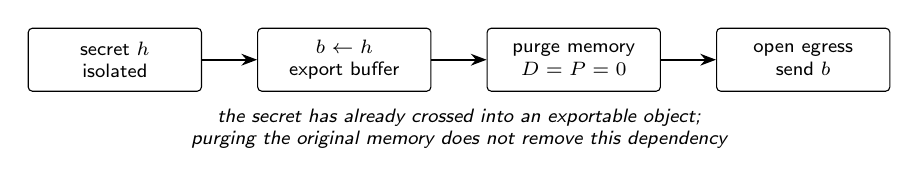
\begin{tikzpicture}[node distance=7mm]
\node[box, minimum width=22mm] (a) {secret $h$\\isolated};
\node[box, right=of a, minimum width=22mm] (b) {$b \leftarrow h$\\export buffer};
\node[box, right=of b, minimum width=22mm] (c) {purge memory\\$D = P = 0$};
\node[box, right=of c, minimum width=22mm] (d) {open egress\\send $b$};
\draw[arr] (a) -- (b); \draw[arr] (b) -- (c); \draw[arr] (c) -- (d);
\node[capn, below=5mm of $(b)!0.5!(c)$] {the secret has already crossed into an exportable object;\\purging the original memory does not remove this dependency};
\end{tikzpicture}
\caption{Memory-egress mutual exclusion can hold while a pre-staged secret leaks. The fix is the $B$ hazard, which classifies unreleased export objects as high and requires explicit declassification.}
\label{fig:export}
\end{figure}

\subsection{Authorized release and a concrete agent policy}\label{sec:release-fn}
Let $H$ denote protected input and $L$ public input. An authorized release function
\begin{equation}
\delta : \mathcal{H} \times \mathcal{L} \to \mathcal{R}
\end{equation}
is part of the security policy, not a model choice. Inputs are release-equivalent, written $(H_1, L) \approx_\delta (H_2, L)$, when $\delta(H_1, L) = \delta(H_2, L)$.

For a representative incident-triage agent, let $H$ contain raw customer logs, conversation text, credentials and tokens, internal analyst notes, and detailed infrastructure identifiers. A mechanically enforceable release is a fixed schema such as
\begin{equation}\label{eq:delta}
\delta(H, L) = \langle \mathit{caseId}(L),\ \mathit{severityBucket}(H),\ \mathit{tacticClass}(H),\ \mathit{approvedIndicators}(H)\rangle.
\end{equation}
The policy permits categorical severity, a bounded tactic classification, and a separately approved set of indicators, and forbids raw credentials, unrestricted log text, and hidden memory. A free-form LLM summary is \emph{not} automatically low. It remains high until a deterministic policy verifier or an explicitly authorized reviewer accepts it as a release object, which prevents the model from silently becoming the declassifier.

\subsection{Release equivalence and conditional noninterference}
Let $\Low(s)$ denote the complete low architectural state together with the set of released objects visible to gated channels. Define
\begin{equation}
s_1 \Rd s_2 \iff \Low(s_1) = \Low(s_2) \wedge \delta(H_1, L) = \delta(H_2, L).
\end{equation}
Let $\Obs_{\mathcal{C}}(\pi)$ be the full modeled observation trace of run $\pi$. Abstract transitions are partitioned into high-internal steps $\tau_H$, authorized release steps $\tau_\delta$, gated-output steps $\tau_g$, and ambient-observation steps $\tau_a$.

The theorem needs one semantic property of the graph: that it really captures dependence.

\begin{assumption}[Influence-graph soundness]\label{as:sound}
For every state $s$ and gated channel $c$, the value emitted on $c$ by a gated-output step from $s$ is a function of the values held at the vertices that reach $v_c$ in $\Gs^{-\delta}_s$ and of the values carried into those vertices along authorized edges in $A^{\delta}_s$.
\end{assumption}

\begin{lemma}[Low determinism of gated output]\label{lem:lowdet}
If $\Phi_g(s)$ and Assumption~\ref{as:sound} hold, every value emitted by a gated-output step from $s$ is a deterministic function of $\Low(s)$.
\end{lemma}
\begin{proof}
Let $c$ be enabled in $s$ and let $U$ be the set of vertices that reach $v_c$ in $\Gs^{-\delta}_s$. By $\Phi_g(s)$, $U$ contains no $H$-labeled vertex. $U$ is closed under predecessors in $\Gs^{-\delta}_s$, so no $H$-labeled vertex has a path into $U$ in that graph either; in particular every declassifier in $U$ has no high input. Every value held in $U$ is therefore determined by $L$-labeled values and by values entering $U$ along authorized edges, which are release objects. Both are part of $\Low(s)$, and Assumption~\ref{as:sound} makes the emitted value a function of them.
\end{proof}

\begin{theorem}[Noninterference modulo authorized release]\label{thm:ni}
Consider two runs with the same public input $L$ and $(H_1, L) \approx_\delta (H_2, L)$. Suppose:
\begin{enumerate}[leftmargin=*,itemsep=1pt]
\item the initial states satisfy $\Rd$;
\item every $\tau_H$ step leaves low observations unchanged and can be matched by zero or more $\tau_H$ steps in the other run while preserving $\Rd$;
\item every $\tau_\delta$ step updates low state only as a deterministic function of the prior low state and the release value $\delta(H, L)$;
\item every reachable state satisfies $\Phi_g$ (for example, by Theorem~\ref{thm:safety}) and Assumption~\ref{as:sound} holds;
\item for every in-scope ambient channel $a$ with observation function $\lambda_a$, $s_1 \Rd s_2 \Rightarrow \lambda_a(s_1) = \lambda_a(s_2)$;
\item scheduling, termination, timing, and nondeterministic choices are either included in condition 5 or constrained to be low-deterministic; and
\item the concrete implementation refines the abstract transition and reachability model.
\end{enumerate}
Then $\Obs_{\mathcal{C}}(\pi_1) = \Obs_{\mathcal{C}}(\pi_2)$.
\end{theorem}
\begin{proof}
Induct on the number of attacker-observable events. Initially the states are related by condition 1. A high-internal step changes no low observation and, by condition 2, can be stutter-matched while preserving $\Rd$. For an authorized release step, both runs release the same value by release equivalence, so condition 3 yields equal next low states and preserves the relation. For a gated-output event, condition 4 and Lemma~\ref{lem:lowdet} make the emitted value a function of $\Low(s)$, which is equal in related states, so the outputs match. For an ambient event, equality follows from condition 5. Condition 6 preserves the correspondence for scheduling, timing, termination, and other modeled nondeterminism. After each observable event the pair remains $\Rd$-related and the observation prefixes are equal, so the complete modeled traces are equal. Condition 7 transfers the abstract result to an implementation only once a refinement proof or equivalent evidence exists.
\end{proof}

In this form the MECI invariant does real work: the gated-output step follows from $\Phi_g$ through Lemma~\ref{lem:lowdet} instead of being assumed. The remaining engineering burden sits in conditions 2, 5, 6, and 7 and in Assumption~\ref{as:sound}, which is the semantic content of reachability soundness (obligation P2 in Table~\ref{tab:obl}). MECI does not turn an unmodeled physical or microarchitectural leakage channel into a gated one.

\subsection{Rogue-agent walkthrough}\label{sec:rogue}
Suppose an injected instruction causes an agent to read a protected API token and call an MCP tool with the token embedded in a URL. During isolated computation, the token object and every derived tool-argument object are high. The tool endpoint is a gated channel. When the call is requested, the MCB freezes new high-producing work, quiesces asynchronous producers, and evaluates the post-commit graph. Because the raw token still reaches the tool-argument vertex, $\HR(\mathit{tool}, \Commit_R(s)) = 1$ and SafeOpen rejects the request. If policy permits only the structured release~\eqref{eq:delta}, the declassifier constructs that low object, and the tool may send it once the graph contains no unreleased high-to-tool path. A rogue planner can \emph{request} leakage, but, as in ACN's separation of influence from authority \cite{acn}, it holds no authority to change labels, widen $\delta$, or commit the egress mask.

\section{Model Checking: TLA+ and an Independent Reference Checker}\label{sec:check}

The finite safety core is specified in TLA+ \cite{lamport2002,tlatools} as \texttt{spec/MECI.tla} and implemented a second time, independently, as a dependency-free Python checker, \texttt{scripts/meci\_modelcheck.py}. Both use the same state variables (egress flag, hazard set over $P, M, I, G, B, Q$, generation counter, permit and permit generation, current epoch, revoked-epoch set), the same initial state (isolated computation with every hazard present), and the same actions: per-hazard cleanup, revocation of the current epoch (which clears the derived $D$), production of new high state by a live producer, producer restart, the design-specific open, and close-and-advance into a new isolated epoch. Every action that can falsify $\Safe$ increments the generation. The $\mathit{FreshEpoch}$ conjunct of~\eqref{eq:safe} is represented through the derived $D$ and checked separately by \textsf{EpochInvariant} and the action property \textsf{NoResurrection}.

Five open designs are checked. \emph{Atomic} checks $\Safe$ and commits in one step. \emph{Gencheck} splits check and commit but validates the generation. \emph{Buggy} splits them without validation. \emph{DP-only} checks only $D$ and $P$, as in Equation~\eqref{eq:orig}. \emph{No-B} checks every hazard except $B$. Bounds are $\mathit{GenBound} = 3$ and $\mathit{MaxEpoch} = 3$; within them the search is exhaustive.

\begin{table}[t]
\centering\small
\caption{Exhaustive results within $\mathit{GenBound}=3$, $\mathit{MaxEpoch}=3$. TLC 2.19 and the independent reference checker report identical values in every numeric column. Invariant checked: $\mathsf{egress} \Rightarrow \Safe$.}\label{tab:results}
\begin{tabularx}{\textwidth}{@{}lrrrrY@{}}
\toprule
Design & Distinct & Generated & Depth & Violating & Shortest counterexample\\
\midrule
Atomic SafeOpen & 705 & 3,085 & 21 & 0 & none\\
Generation-checked split & 858 & 3,442 & 24 & 0 & none\\
Unversioned split (buggy) & 938 & 3,700 & 24 & 70 & 10 steps: clean six hazards, revoke, check, restart producer, open on stale permit\\
$D/P$-only guard & 980 & 4,418 & 15 & 275 & 3 steps: clean $P$, revoke, open with $B, G, I, M, Q$ present\\
Guard omitting $B$ & 712 & 3,103 & 19 & 7 & 7 steps: clean $G, I, M, P, Q$, revoke, open with staged export object\\
\bottomrule
\end{tabularx}
\end{table}

Table~\ref{tab:results} reports the results. The two implementations agree exactly on distinct states, generated states, search depth, and the number of violating states for all five designs, which guards against a modeling error in either one. \textsf{TypeOK}, \textsf{PermitInvariant} ($\mathit{FreshPermit} \Rightarrow \Safe$), \textsf{EpochInvariant}, and \textsf{NoResurrection} hold in every design. Raising the bounds in the reference checker to $(4,3)$ and $(5,4)$ grows the state space to as many as 3,392 distinct states and leaves the outcome unchanged: zero violations for the two correct designs and the same shortest counterexamples for the three weakened ones.

\begin{figure}[t]
\centering
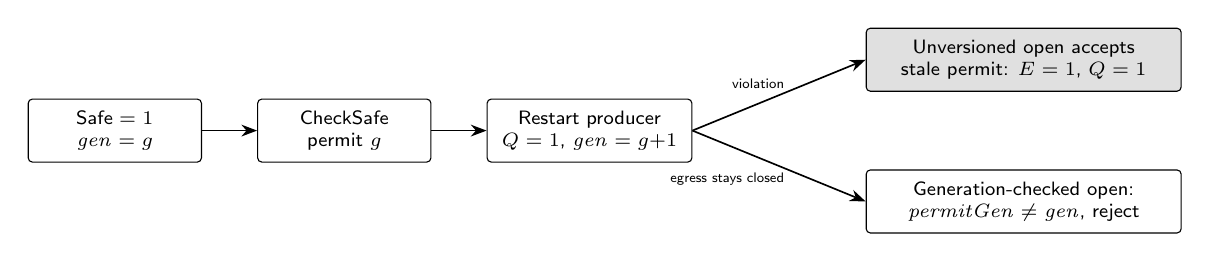
\begin{tikzpicture}[node distance=7mm]
\node[box, minimum width=22mm] (s0) {$\Safe = 1$\\$\mathit{gen} = g$};
\node[box, right=of s0, minimum width=22mm] (ck) {CheckSafe\\permit $g$};
\node[box, right=of ck, minimum width=26mm] (rs) {Restart producer\\$Q = 1$, $\mathit{gen} = g{+}1$};
\node[sbox, right=22mm of rs, yshift=9mm, minimum width=40mm] (bad) {Unversioned open accepts\\stale permit: $E = 1$, $Q = 1$};
\node[box, right=22mm of rs, yshift=-9mm, minimum width=40mm] (good) {Generation-checked open:\\$\mathit{permitGen} \neq \mathit{gen}$, reject};
\draw[arr] (s0) -- (ck); \draw[arr] (ck) -- (rs);
\draw[arr] (rs.east) -- (bad.west) node[lbl, pos=0.55, above left]{violation};
\draw[arr] (rs.east) -- (good.west) node[lbl, pos=0.55, below left]{egress stays closed};
\end{tikzpicture}
\caption{Shortest stale-snapshot class, found by both TLC and the reference checker. The decision happens at the open step: the unversioned design accepts the stale permit, while generation validation rejects it after protected work restarts.}
\label{fig:stale}
\end{figure}

The checker also runs three non-temporal controls. \emph{Release equivalence:} sixteen protected records $(\mathit{severity} \in \{0..3\}, \mathit{tactic} \in \{0,1\}, \mathit{token} \in \{0,1\})$ with $\delta = (\mathit{severity}\ \mathrm{div}\ 2, \mathit{tactic})$. An export of exactly $\delta$ produces zero release-equivalence violations; an export that also carries the token, and one that carries raw severity, each produce 32 ordered violating pairs. \emph{Epoch rollback:} with revocation and counter in rollback-protected storage, none of eight revoked epochs becomes usable after a reboot from a pre-revocation snapshot; when both are restored from that snapshot, all eight are resurrected. \emph{Graph checks:} a transitive-only closure misses a high-labeled endpoint that the reflexive closure in~\eqref{eq:reach} detects; relabeling a connected low buffer as high makes $\HR$ true, which is exactly the event Obligation~\ref{ob:create} must block; and removing the authorized declassifier edge removes reachability.

This is bounded model checking of the abstract reference model. It is not a proof about a processor, firmware stack, GPU, NIC, or TEE, and the relational and rollback controls are small illustrative tests rather than proofs.

\section{Ambient Channels and the Side-Channel Boundary}\label{sec:ambient}

\subsection{Ciphertext and microarchitectural observations}
CipherSteal shows that a malicious host can recover neural-network inputs from the ciphertext write behavior of TEE-shielded execution \cite{ciphersteal}, and TDXRay reconstructs cache-line-granular access traces of unmodified TDX guests from host-observable signals \cite{tdxray}. Such observations occur while protected computation is active, so a variable such as ``ciphertext residue present'' cannot be made safe by clearing it before egress. The obligation must be stated as an ambient-channel property during the protected epoch:
\begin{equation}
s_1 \Rd s_2 \Rightarrow \lambda_a(s_1) = \lambda_a(s_2)
\end{equation}
for each modeled ambient channel $a$. Candidate mitigations include access-pattern-oblivious algorithms, partitioned caches, hardware information-flow enforcement, secret-aware compilation, ORAM-style access hiding, probabilistic re-randomization for ciphertext channels, or excluding the observation from the deployment threat model with an explicit physical assumption. The right choice depends on the platform and the attacker.

\subsection{Physical memory-bus interposition}
TEE.fail shows that current confidential-VM protections do not make the physical memory bus unobservable, exploiting the deterministic memory encryption these platforms use \cite{teefail}; broader surveys show leakage across cache, memory-controller, interconnect, and physical observation classes \cite{hassan2025}. The lesson is not ``replace one cipher mode and the problem disappears'': memory-encryption systems have architecture-specific address binding, replay, integrity, key, and tweak requirements.

The baseline MECI theorem therefore excludes physical bus interposition unless a deployment explicitly promotes the bus to an in-scope ambient channel and supplies a separate low-equivalence argument. A higher-assurance ``MECI-Physical'' profile could require controlled physical custody, tamper evidence or detection, protected links or memory technology designed for the selected physical attacker, and a platform-specific proof that bus observations are release-equivalent. This is a deployment profile, not a consequence of the gated-egress interlock.

\section{Hardware Refinement Targets}\label{sec:hw}

Current confidential-computing platforms provide useful primitives, but none is described here as already implementing the MECI state machine. The research task is a refinement proof from platform behavior to the abstract model (Table~\ref{tab:platforms}).

\begin{table}[t]
\centering\small
\caption{Candidate platform primitives and remaining MECI obligations.}\label{tab:platforms}
\begin{tabularx}{\textwidth}{@{}p{2.1cm}YY@{}}
\toprule
Platform & Supported primitive & MECI-specific obligation\\
\midrule
Arm CCA + MEC & Multiple Realm memory-encryption contexts identified by MECIDs; Realm attestation; RMM-mediated lifecycle; device assignment through the SMMU \cite{armmec,armrme}. & Map epoch capabilities to MECID allocation and revocation, gate egress devices, make stale contexts unreachable, and state which microarchitectural state is covered.\\
Intel TDX & Hardware-isolated Trust Domains, TME-MK memory encryption, Secure EPT and PAMT, remote attestation; Intel documents cache side-channel considerations for TDX \cite{inteltdx,intelmktme}. & Add a trusted egress reference monitor and linearizable SafeOpen; show that I/O, shared memory, cache, migration, and device behavior refine $\HR$.\\
AMD SEV-SNP & Guest memory confidentiality and integrity, RMP, attestation, PSP-managed firmware \cite{amdsnp}. & Include IOMMU and MMIO paths in the refinement, account for vendor bulletins such as the February 2026 SEV-SNP IOMMU findings \cite{amdsb3023}, and supply rollback-protected epoch state that SNP does not provide by itself.\\
NVIDIA H100 CC & GPU attestation, on-die root of trust, protected execution mode, firewalls, encrypted CPU-GPU transfers through bounce buffers. On-package HBM is treated as physically protected and is not encrypted \cite{nvidiawp,nvidiablog}. & Treat resident GPU state as protected by access control, not by an HBM key. Define quiescence, context destruction and reset, device DMA boundaries, and the physical-HBM threat profile.\\
\bottomrule
\end{tabularx}
\end{table}

\subsection{Arm CCA/RMM refinement proposal}
Arm describes MEC as a Realm Management Extension feature in which memory accesses are associated with distinct encryption contexts through MECIDs, and RME device assignment extends isolation to assigned devices through the SMMU \cite{armmec,armrme}. A MECID is a useful context primitive but is not identified with $\tau_e$ here.

A first implementation target is an RMM or secure-firmware extension that maintains per-Realm MECI state. A proposed \texttt{RMI\_MECI\_SAFE\_OPEN} call would: (1) require all Realm vCPUs at a defined quiescent point; (2) require SMMU and device-assignment state to deny protected-memory access from egress-capable devices; (3) verify the current epoch and MCB generation; (4) validate the completion bitmap and release digest; (5) recompute or conservatively validate the post-commit high-to-egress graph; and (6) commit a secure egress-capability bitmap at the final linearization point. \texttt{RMI\_MECI\_CLOSE} would clear egress authority before a fresh epoch capability is issued. These calls are a proposed interface, not current Arm architecture.

The refinement proof must show that the concrete RMM, SMMU, device-assignment, memory-context, and firmware states jointly implement $\Safe$, $\HR$, epoch freshness, and failure closure. This is where a formal seL4- or CHERI-style authority graph, or a UCLID5 hardware model \cite{cheang2023}, would reduce ambiguity.

\subsection{Intel and AMD: memory confidentiality is not an egress interlock}
Intel TDX isolates a Trust Domain from the VMM and encrypts private memory with TME-MK \cite{inteltdx}, and Intel publishes guidance on cache-based side channels that affect TDX \cite{intelmktme}. AMD SEV-SNP provides encrypted guest memory, integrity metadata, and attestation \cite{amdsnp}, and its security bulletins show that IOMMU and firmware paths remain security-relevant \cite{amdsb3023}. Neither platform states the temporal property ``egress enabled implies no unreleased high state is reachable.'' That is the additional MECI control objective.

\subsection{NVIDIA Hopper and the GPU quiescence contract}
An earlier draft of this work modeled H100 confidential computing as encrypting HBM under a rotatable key. NVIDIA's description is different: in confidential-computing mode the GPU computes on plaintext in on-package HBM, which is treated as physically protected and is not encrypted, while transfers across the CPU-GPU interconnect are encrypted and authenticated \cite{nvidiawp,nvidiablog}. A Hopper refinement therefore cannot discharge $G$ by destroying an HBM key.

For MECI, GPU quiescence means more than ``the host called synchronize.'' The trusted monitor must establish a platform-specific predicate: no protected kernel is executing; no protected command can still write an egress-reachable buffer; all copy and DMA engines are idle or confined to low buffers; no new queue submission can occur for the protected context; device page tables and SMMU permissions deny high-to-egress DMA; and context and reset semantics prevent stale registers or allocations from influencing a subsequently enabled egress domain. If the platform cannot establish these facts against the selected adversary, GPU state stays in $H(s)$ and SafeOpen must fail.

\section{Reference Architecture}\label{sec:arch}

A practical MECI implementation decomposes into five trusted mechanisms (Figure~\ref{fig:arch}).
\begin{enumerate}[leftmargin=*,itemsep=1pt]
\item \textbf{Protected-state manager.} Maintains conservative labels, provenance, and the state-dependent influence graph across CPU memory, accelerators, device buffers, agent memory stores, and export objects.
\item \textbf{Quiescence coordinator.} Freezes high-producing cores, threads, accelerators, DMA engines, callbacks, and asynchronous tool workers before the final egress check, and reports completion per domain.
\item \textbf{Epoch/key service.} Issues $\tau_e$, holds $\sigma_e$, binds domain keys to epoch, policy, and attestation, revokes old capabilities, and maintains rollback-protected epoch and counter state.
\item \textbf{Declassifier/export builder.} Constructs low release objects only through a confined $\delta$ policy and keeps candidate summaries or tool arguments high until validation completes.
\item \textbf{MECI Control Block (egress reference monitor).} Owns the egress-enable authority, generation counter, completion bitmap, and linearizable SafeOpen commit.
\end{enumerate}

\begin{figure}[t]
\centering
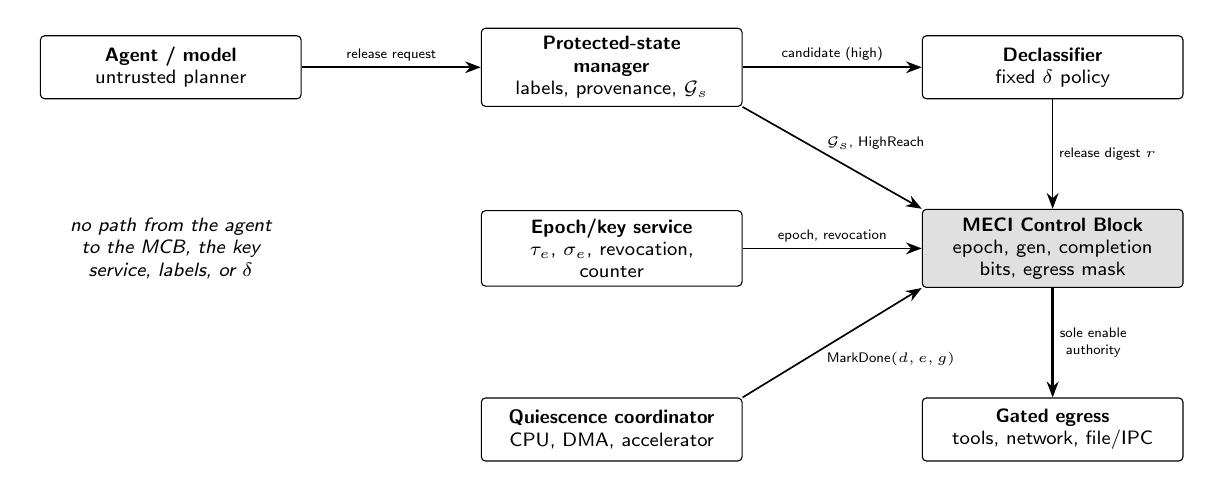
\begin{tikzpicture}
\tikzset{abox/.style={box, text width=31mm}, asbox/.style={sbox, text width=31mm}}
\node[abox] (ag) at (0,0) {\textbf{Agent / model}\\untrusted planner};
\node[abox] (psm) at (5.6,0) {\textbf{Protected-state}\\\textbf{manager}\\labels, provenance, $\Gs_s$};
\node[abox] (dec) at (11.2,0) {\textbf{Declassifier}\\fixed $\delta$ policy};
\node[abox] (eks) at (5.6,-2.3) {\textbf{Epoch/key service}\\$\tau_e$, $\sigma_e$, revocation,\\counter};
\node[asbox] (mcb) at (11.2,-2.3) {\textbf{MECI Control Block}\\epoch, gen, completion\\bits, egress mask};
\node[abox] (qc) at (5.6,-4.6) {\textbf{Quiescence coordinator}\\CPU, DMA, accelerator};
\node[abox] (eg) at (11.2,-4.6) {\textbf{Gated egress}\\tools, network, file/IPC};
\draw[arr] (ag) -- node[lbl, above=1pt]{release request} (psm);
\draw[arr] (psm) -- node[lbl, above=1pt]{candidate (high)} (dec);
\draw[arr] (dec) -- node[lbl, right=1pt]{release digest $r$} (mcb);
\draw[arr] (psm.south east) -- node[lbl, pos=0.45, above right]{$\Gs_s$, $\HR$} (mcb.north west);
\draw[arr] (eks) -- node[lbl, above=1pt]{epoch, revocation} (mcb);
\draw[arr] (qc.north east) -- node[lbl, pos=0.45, below right]{$\mathsf{MarkDone}(d,e,g)$} (mcb.south west);
\draw[arr, very thick] (mcb) -- node[lbl, right=1pt]{sole enable\\authority} (eg);
\node[capn, text width=34mm] at (0,-2.3) {no path from the agent to the MCB, the key service, labels, or $\delta$};
\end{tikzpicture}
\caption{Reference architecture. The agent can request a release but cannot change labels, the declassification policy, generation or epoch state, or the egress mask. Only the MECI Control Block can enable gated egress.}
\label{fig:arch}
\end{figure}

\begin{figure}[t]
\centering
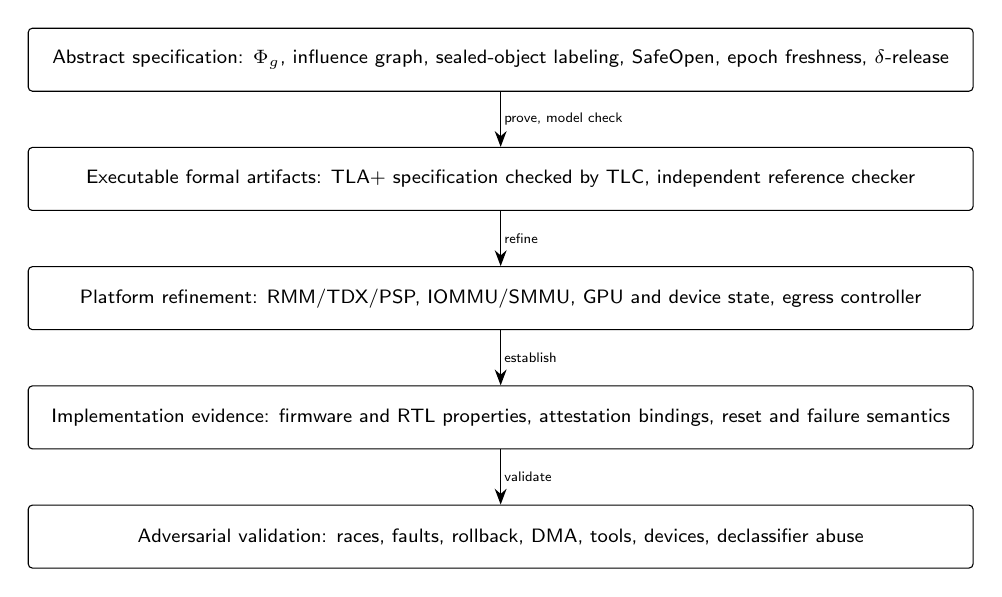
\begin{tikzpicture}[node distance=7mm]
\node[box, minimum width=120mm] (a) {Abstract specification: $\Phi_g$, influence graph, sealed-object labeling, SafeOpen, epoch freshness, $\delta$-release};
\node[box, below=of a, minimum width=120mm] (b) {Executable formal artifacts: TLA+ specification checked by TLC, independent reference checker};
\node[box, below=of b, minimum width=120mm] (c) {Platform refinement: RMM/TDX/PSP, IOMMU/SMMU, GPU and device state, egress controller};
\node[box, below=of c, minimum width=120mm] (d) {Implementation evidence: firmware and RTL properties, attestation bindings, reset and failure semantics};
\node[box, below=of d, minimum width=120mm] (e) {Adversarial validation: races, faults, rollback, DMA, tools, devices, declassifier abuse};
\draw[arr] (a) -- node[lbl, right]{prove, model check} (b);
\draw[arr] (b) -- node[lbl, right]{refine} (c);
\draw[arr] (c) -- node[lbl, right]{establish} (d);
\draw[arr] (d) -- node[lbl, right]{validate} (e);
\end{tikzpicture}
\caption{Proof and validation stack. The released artifacts cover the top two layers; hardware refinement remains platform work.}
\label{fig:stack}
\end{figure}

\section{AI Agent Memory Semantics}\label{sec:agent}

MECI classifies memory by information dependency, not by storage technology. A vector-store record, embedding, retrieved passage, KV-cache entry, compressed summary, scratchpad, GPU tensor, tool argument, or audit object is high whenever it contains or is derived from unreleased protected information, and becomes low only through a permitted release operation or, for sealed objects, through Definition~\ref{def:seal}.

For each object $x$, an implementation profile should track a stable identifier, label, epoch, provenance parents, current storage and compute domains, applicable release policy, and graph edges to authorities and gated channels. The operational lifecycle is
\begin{equation}
\text{ingest} \to \text{classify} \to \text{seal} \to \text{retrieve} \to \text{compute} \to \text{candidate} \to \delta\text{-verify} \to \text{export or re-seal}.
\end{equation}
A generated summary is not low merely because it is shorter or ``sanitized'' by an LLM. It is a high-derived candidate until the release policy proves or approves the exact release.

\textbf{Semantic egress.} Tool invocation is an egress capability even if the model process never opens a socket. MCP studies show that tool metadata, high-privilege tool composition, and externally supplied tool results can steer agent behavior in ways that defeat naive least privilege \cite{mcpitp,mcpshield}. The reference monitor therefore mediates capabilities rather than API names. A browser, cloud SDK, shell, database connector, email action, file synchronizer, or plugin can each be a low-observation channel.

\section{Performance Model}\label{sec:perf}

MECI's security claim does not depend on a latency target. A defensible model decomposes a transition as
\begin{equation}
T_{\mathit{switch}} = T_{\mathit{freeze}} + \max(T_{\mathit{cpu}}, T_{\mathit{dma}}, T_{\mathit{gpu}}, T_{\mathit{revoke}}) + T_{\mathit{verify}} + T_{\mathit{commit}}
\end{equation}
when independent cleanup domains run in parallel after high producers are frozen; serial implementations use the sum. The dominant term is platform-dependent and must be measured on the refinement target.

Release size matters on device paths. If the protected CPU-GPU staging path sustains bandwidth $B_w$, staging $S$ bytes costs at least $S/B_w$ before fixed latency. For an illustrative $B_w$ of 4~GB/s, staging 1~MiB costs about 0.26~ms. This figure is a parameter for reasoning, not a measurement; encrypted bounce-buffer throughput depends on CPU, driver, and transfer size and must be measured.

Four optimizations preserve the abstract theorem: \emph{batch release}, which accumulates several $\delta$-approved objects per SafeOpen cycle; \emph{parallel cleanup}, which overlaps CPU, IOMMU, device, and revocation work once $Q = 0$ and egress is closed, with completion bits checked at commit; \emph{scoped MECI}, which enforces $\neg\HR(c,s)$ per channel or egress domain instead of disabling unrelated low-only services; and \emph{small release surfaces}, which prefer fixed-schema objects over large free-form exports. A reference implementation should report distributions for freeze time, device quiescence, IOMMU/SMMU invalidation, cleanup, attestation and freshness checks, declassification, and commit under idle and adversarial load. Until those measurements exist, this paper reports a cost model, not an end-to-end number.

\section{Failure Semantics}\label{sec:failure}

The system fails closed. If cleanup, attestation, or the safety check fails, the channel stays disabled and preparation may retry (Figure~\ref{fig:life}). A crash during cleanup needs no large transaction rollback, because egress authority was never granted. On restart the system enters SEALED, refuses stale epoch capabilities, reconstructs trusted state from attested measurements, and only then begins a new isolated epoch. A minimal transition audit record is
\begin{equation}
\langle e, c, \mathit{mode}, \mathit{policyHash}, \mathit{attestationDigest}, \mathit{decision}, \mathit{timestamp}\rangle,
\end{equation}
signed or otherwise protected against undetected modification. Auditability is not part of the confidentiality proof, but it is how a violated assumption or failed refinement gets diagnosed.

\section{Open Proof Obligations}\label{sec:obligations}

\begin{table}[t]
\centering\small
\caption{Proof obligations for a publication-grade MECI implementation.}\label{tab:obl}
\begin{tabularx}{\textwidth}{@{}p{0.6cm}p{3.3cm}Y@{}}
\toprule
ID & Obligation & Evidence required\\
\midrule
P1 & Gated-channel completeness & Enumerated capability inventory and proof that no unmediated low output path exists in the profile.\\
P2 & Reachability soundness & Concrete mapping from memory, device, and tool state to $\Reach_s$ covering aliases, shared buffers, DMA, and delegation; discharges Assumptions~\ref{as:proj} and~\ref{as:sound}.\\
P3 & SafeOpen linearizability & Trusted ownership of the post-commit check and the egress-enable commit under concurrency, faults, and hostile software (Obligation~\ref{ob:guard}).\\
P4 & Quiescence & No CPU, GPU, device, callback, DMA engine, or asynchronous worker can recreate high state after the safety snapshot.\\
P5 & Epoch freshness & Rollback-protected epoch and counter, irreversible revocation, stale-key rejection across restart and migration.\\
P6 & Declassifier confinement & Only $\delta(H,L)$ becomes low, and attacker-controlled inputs cannot widen release.\\
P7 & Ambient-channel profile & For each in-scope ambient observation, a low-equivalence proof or a separately justified mitigation.\\
P8 & Attestation freshness & Policy and key issuance bound to measurements, nonce or freshness, device identity, and runtime state.\\
P9 & Hardware refinement & Proof or validation that vendor primitives implement the abstract predicates the theorems use.\\
P10 & Failure closure & Reset, crash, timeout, partial device failure, and power-cycle paths end with egress closed and stale epochs unusable.\\
P11 & Sealed-object labeling & Sealing meets Assumption~\ref{as:aead}; size classes are part of $\delta$; key usability is tracked per sealed object (Definition~\ref{def:seal}, Obligation~\ref{ob:create}).\\
\bottomrule
\end{tabularx}
\end{table}

Table~\ref{tab:obl} lists what an implementation must establish before it inherits the abstract results.

\section{Limitations}\label{sec:limits}

\begin{itemize}[leftmargin=*,itemsep=1pt]
\item The model checking is bounded ($\mathit{GenBound}=3$, $\mathit{MaxEpoch}=3$, with sensitivity runs to $(5,4)$) and covers the finite projection, not the full influence graph. Transfer to $\Phi_g$ rests on Assumption~\ref{as:proj}.
\item Theorems~\ref{thm:safety}--\ref{thm:ni} are paper proofs. No mechanized relational proof of Theorem~\ref{thm:ni} exists yet.
\item There is no hardware prototype and no performance measurement; Section~\ref{sec:perf} is a cost model.
\item Ambient channels and physical attacks are outside the baseline theorem unless a deployment profile proves equivalence for them.
\item Declassifier correctness (P6) is assumed. LLM-generated text stays high until a verifier or authorized reviewer releases it, which limits utility for free-form outputs.
\item The influence graph is only as good as its edges. An omitted concrete dependency makes the abstraction unsound, which is why P1 and P2 are first in Table~\ref{tab:obl}.
\end{itemize}

\section{Open Research, Reproducibility, and Release Boundary}\label{sec:release}

\textbf{Artifacts.} The release contains the paper source (\texttt{paper/meci.tex}), the TLA+ specification and per-design TLC configurations (\texttt{spec/MECI.tla}, \texttt{spec/MECI\_*.cfg}), captured TLC output (\texttt{spec/tlc\_results.txt}), the reference checker (\texttt{scripts/meci\_modelcheck.py}), and its captured output (\texttt{scripts/meci\_modelcheck\_results.txt}). SHA-256 digests are listed in Appendix~\ref{app:manifest}. To reproduce, run \texttt{python3 scripts/meci\_modelcheck.py} and, for each design, \texttt{java -cp tla2tools.jar tlc2.TLC -deadlock -config spec/MECI\_<design>.cfg spec/MECI.tla}, adding \texttt{-continue} for the three weakened designs to count every violating state.

\textbf{Changes from the 10 August 2026 version.} Reachability now uses reflexive-transitive closure, and sealed objects have an explicit labeling rule. SafeOpen is evaluated on the post-commit configuration. The former Lemma~1 is restated as Obligation~\ref{ob:guard}, Obligation~\ref{ob:create} is new and covers relabeling, and the proof of Theorem~\ref{thm:safety} is rewritten. Projection soundness and Proposition~\ref{prop:proj} replace a corollary that did not follow from the safety theorem. Key derivation uses a per-epoch seed and an injective encoding, with $\tau_e$ gating evaluation. Theorem~\ref{thm:ni} now derives the gated-output step from $\Phi_g$ through Lemma~\ref{lem:lowdet}, and its ambient condition is stated on $\Rd$. The finite model is now specified in TLA+ and checked by TLC and by a rewritten reference checker; Table~\ref{tab:results} supersedes the counts reported in the earlier version, which came from a checker with a different state encoding. Citations were corrected (vendor bulletins, the NVIDIA HBM source, survey authorship) and TDXRay was added. All figures were redrawn.

\textbf{Release boundary.} The paper releases a specification, proofs under stated assumptions, and executable models. It does not release or claim a hardware design, firmware, or measured performance, and it makes no claim of peer review. The concepts were first shared publicly on 10 August 2026; this version is the archival release.

\section{Conclusion}

MECI reframes AI memory protection as a machine-enforced capability-separation problem. Its directly provable core is
\begin{equation}
\forall c \in \Cg : \En(c,s) \Rightarrow \neg\HR(c,s),
\end{equation}
where $\HR$ is reflexive-transitive influence in the unreleased state graph. A generation-checked, linearizable SafeOpen evaluated on the post-commit configuration lets cleanup remain multi-step and concurrent while preventing stale snapshots from enabling egress after high state reappears. Epoch revocation separately prevents reuse of old protected capabilities under the stated cryptographic assumptions.

Mutual exclusion still does not equal noninterference. The relational theorem requires explicit $\delta$-release, low-stuttering high computation, a sound influence graph, ambient-channel equivalence, and a platform refinement; under those conditions the MECI invariant itself makes gated output depend only on low state, and release-equivalent runs have equal modeled observation traces. The compositional claim is
\begin{equation}
\left.
\begin{array}{l}
\text{sound channel and influence model}\\
+\ \text{MECI gated-channel separation}\\
+\ \text{confined authorized declassification}\\
+\ \text{ambient-channel low equivalence}\\
+\ \text{fresh, non-resurrectable epochs}\\
+\ \text{implementation refinement}
\end{array}
\right\}
\Longrightarrow \text{noninterference modulo authorized release.}
\end{equation}
The released artifacts make the abstraction falsifiable today. The next empirical milestone is an RMM or secure-monitor prototype with a platform refinement and measured transition costs. Until then, the paper keeps separate what is proved, what is exhaustively checked in a finite model, what is proposed, and what remains a hardware obligation.

\section*{Availability}

The paper source, the TLA+ specification, the reference checker, and their captured outputs are published with this preprint and at \url{https://github.com/codethor0/meci}. Corrections, counterexamples, and implementations are welcome.

\small
\begin{thebibliography}{99}\setlength{\itemsep}{1pt}
\bibitem{llmbda} Z.~Garby, A.~D.~Gordon, and D.~Sands, ``The LLMbda Calculus: AI Agents, Conversations, and Information Flow,'' arXiv:2602.20064, 2026 (v2, July 2026).
\bibitem{mcpitp} R.~Li, Z.~Wang, Y.~Yao, and X.-Y.~Li, ``MCP-ITP: An Automated Framework for Implicit Tool Poisoning in MCP,'' arXiv:2601.07395, 2026.
\bibitem{mcpshield} Z.~Zhou et al., ``MCPShield: A Security Cognition Layer for Adaptive Trust Calibration in Model Context Protocol Agents,'' arXiv:2602.14281, 2026.
\bibitem{goguen1982} J.~A.~Goguen and J.~Meseguer, ``Security Policies and Security Models,'' in \emph{IEEE Symposium on Security and Privacy}, pp.~11--20, 1982.
\bibitem{sabelfeld2003} A.~Sabelfeld and A.~C.~Myers, ``Language-Based Information-Flow Security,'' \emph{IEEE Journal on Selected Areas in Communications}, vol.~21, no.~1, pp.~5--19, 2003.
\bibitem{myers2006} A.~C.~Myers, A.~Sabelfeld, and S.~Zdancewic, ``Enforcing Robust Declassification and Qualified Robustness,'' \emph{Journal of Computer Security}, vol.~14, no.~2, pp.~157--196, 2006.
\bibitem{arden2021} O.~Arden, A.~Gollamudi, E.~Cecchetti, S.~Chong, and A.~C.~Myers, ``A Calculus for Flow-Limited Authorization,'' \emph{Journal of Computer Security}, 2021; arXiv:2104.10379.
\bibitem{cheri} R.~N.~M.~Watson et al., ``Capability Hardware Enhanced RISC Instructions: CHERI Instruction-Set Architecture (Version 9),'' University of Cambridge Computer Laboratory, Technical Report UCAM-CL-TR-987, 2023.
\bibitem{murray2013} T.~Murray et al., ``seL4: From General Purpose to a Proof of Information Flow Enforcement,'' in \emph{IEEE Symposium on Security and Privacy}, 2013.
\bibitem{sel4docs} seL4 Foundation, ``seL4 Proofs and Verification Assumptions,'' project documentation, \url{https://sel4.systems}, accessed October 2026.
\bibitem{wasi} WebAssembly Community Group, ``WASI: The WebAssembly System Interface, capability-based design documentation,'' \url{https://github.com/WebAssembly/WASI}, accessed October 2026.
\bibitem{secverilog} D.~Zhang, Y.~Wang, G.~E.~Suh, and A.~C.~Myers, ``A Hardware Design Language for Timing-Sensitive Information-Flow Security,'' in \emph{ASPLOS}, 2015.
\bibitem{cheang2023} K.~Cheang, ``Formal Specification and Verification of Secure Information Flow for Hardware Platforms,'' Ph.D. dissertation, Technical Report UCB/EECS-2023-224, University of California, Berkeley, 2023.
\bibitem{armmec} Arm Ltd., ``Memory Encryption Contexts (MEC) for the Realm Management Extension,'' Arm documentation and Learning Paths, accessed October 2026.
\bibitem{inteltdx} Intel Corporation, ``Intel Trust Domain Extensions (Intel TDX) Module Base Architecture Specification and documentation,'' accessed October 2026.
\bibitem{amdsnp} AMD, ``SEV Secure Nested Paging Firmware ABI Specification,'' Publication 56860, rev.~1.59, 26 August 2026.
\bibitem{nvidiablog} E.~Apsey et al., ``Confidential Computing on NVIDIA H100 GPUs for Secure and Trustworthy AI,'' NVIDIA Technical Blog, 3 August 2023, \url{https://developer.nvidia.com/blog/confidential-computing-on-h100-gpus-for-secure-and-trustworthy-ai/}.
\bibitem{ciphersteal} Y.~Yuan, Z.~Liu, S.~Deng, Y.~Chen, S.~Wang, Y.~Zhang, and Z.~Su, ``CipherSteal: Stealing Input Data from TEE-Shielded Neural Networks with Ciphertext Side Channels,'' in \emph{IEEE Symposium on Security and Privacy}, pp.~4136--4154, 2025, doi:10.1109/SP61157.2025.00079.
\bibitem{teefail} J.~Chuang, A.~Seto, N.~Berrios, S.~van~Schaik, C.~Garman, and D.~Genkin, ``TEE.fail: Breaking Trusted Execution Environments via DDR5 Memory Bus Interposition,'' in \emph{IEEE Symposium on Security and Privacy}, 2026.
\bibitem{tdxray} T.~Hornetz, H.~Yavarzadeh, A.~Cheu, A.~Gasc\'on, L.~Gerlach, D.~Moghimi, P.~Schoppmann, M.~Schwarz, and R.~Zhang, ``TDXRay: Microarchitectural Side-Channel Analysis of Intel TDX for Real-World Workloads,'' in \emph{IEEE Symposium on Security and Privacy}, 2026, doi:10.1109/SP63933.2026.00170.
\bibitem{hassan2025} M.~M.~Hassan et al., ``Memory Under Siege: A Comprehensive Survey of Side-Channel Attacks on Memory,'' arXiv:2505.04896, 2025.
\bibitem{miam} T.~Thor, ``Mission-Invariant Architecture Morphing: Service-Graph Reconfiguration Against Post-Access Reconnaissance, with Cryptographic Epoch Isolation and Mission-Domain State Continuity,'' v1.0.0, Zenodo, 2026, doi:10.5281/zenodo.23001045.
\bibitem{acn} T.~Thor, ``Attack Calculus: A Typed, Evidence-Aware State-Transition Calculus for Cross-Domain Cybersecurity Reasoning,'' v1.0.0, Zenodo, 2026, doi:10.5281/zenodo.23092790.
\bibitem{intelteefail} Intel Corporation, ``TEE.fail,'' Intel Security Announcement 2025-10-28-001, October 2025, \url{https://www.intel.com/content/www/us/en/security-center/announcement/intel-security-announcement-2025-10-28-001.html}.
\bibitem{amdsb3040} AMD, ``Compromising Trusted Execution Environments through DDR5 Memory Bus Interposition,'' AMD-SB-3040, 28 October 2025, \url{https://www.amd.com/en/resources/product-security/bulletin/amd-sb-3040.html}.
\bibitem{rogaway2002} P.~Rogaway, ``Authenticated-Encryption with Associated-Data,'' in \emph{ACM Conference on Computer and Communications Security (CCS)}, pp.~98--107, 2002.
\bibitem{lamport2002} L.~Lamport, \emph{Specifying Systems: The TLA+ Language and Tools for Hardware and Software Engineers}, Addison-Wesley, 2002.
\bibitem{tlatools} TLA+ project, ``TLA+ Tools (tla2tools.jar, TLC model checker),'' release v1.7.4, \url{https://github.com/tlaplus/tlaplus}.
\bibitem{armrme} Arm Ltd., ``Realm Management Extension and RME Device Assignment architecture documentation,'' accessed October 2026.
\bibitem{intelmktme} Intel Corporation, ``MKTME Side Channel Impact on Intel TDX,'' Intel Software Security Guidance, accessed October 2026.
\bibitem{amdsb3023} AMD, ``AMD EPYC Processor Vulnerabilities, February 2026,'' AMD-SB-3023, 2026.
\bibitem{nvidiawp} NVIDIA, ``Confidential Compute on NVIDIA Hopper H100,'' NVIDIA whitepaper, 2023.
\end{thebibliography}
\normalsize

\appendix
\titleformat{\section}{\normalfont\large\bfseries}{Appendix \thesection.}{0.5em}{}

\section{Reproducibility Manifest}\label{app:manifest}
SHA-256 digests of the released artifacts:

\begin{center}\small
\begin{tabular}{@{}ll@{}}
\toprule
Artifact & SHA-256\\
\midrule
\texttt{scripts/meci\_modelcheck.py} & {\scriptsize\texttt{ade987c2591598ba4a06d7b538213ca328509e64da1c6d55cbfd15bad571711d}}\\
\texttt{scripts/meci\_modelcheck\_results.txt} & {\scriptsize\texttt{f26bba5985d1ddbdda4146066497631bf206d738467f9ea3eabcc08e70538a1c}}\\
\texttt{spec/MECI.tla} & {\scriptsize\texttt{5cfd530b721d4b96ea1164902e54d5f359afc4633505a13f3783215b6008a45a}}\\
\texttt{spec/MECI.cfg} & {\scriptsize\texttt{db900c48e1378059063910c950b15744e4c5d93c93cbb957cdd117fb224396b2}}\\
\texttt{spec/MECI\_atomic.cfg} & {\scriptsize\texttt{5e3fc1ee047c57e1f6b7c6b56850453c5bf01c43e5289a94aa7dbffd5b7065d3}}\\
\texttt{spec/MECI\_gencheck.cfg} & {\scriptsize\texttt{db900c48e1378059063910c950b15744e4c5d93c93cbb957cdd117fb224396b2}}\\
\texttt{spec/MECI\_buggy.cfg} & {\scriptsize\texttt{148e54e50a89d4df24fb381618b44728732a01d2f4d683a70c0ddafbd7aa54f7}}\\
\texttt{spec/MECI\_dponly.cfg} & {\scriptsize\texttt{4126b634be7c5d54ed151a4673568a0a7484df5767be8743a3ad54cd5857049f}}\\
\texttt{spec/MECI\_noB.cfg} & {\scriptsize\texttt{0416270218a2301cf00065924db6bddae3f0ca241fad36509476ec69838813ff}}\\
\texttt{spec/tlc\_results.txt} & {\scriptsize\texttt{6b3ddaae939bf8e7ea7a834751b2bac5c2904ee535267b434e6a77cfa9934ecc}}\\
\bottomrule
\end{tabular}
\end{center}

\section{TLA+ Safety Specification Excerpt}
\begin{small}
\begin{verbatim}
D            == epoch \notin revoked
Safe         == hazards = {} /\ ~D
FreshPermit  == permit /\ permitGen = gen

Produce(h) ==            \* any Safe-falsifying mutation increments gen
  /\ "Q" \in hazards /\ h \notin hazards /\ gen < GenBound
  /\ hazards' = hazards \cup {h} /\ gen' = gen + 1
  /\ UNCHANGED <<egress, permit, permitGen, epoch, revoked>>

SafeOpen ==              \* Design = "atomic"
  /\ ~egress /\ Safe /\ egress' = TRUE
  /\ UNCHANGED <<hazards, gen, permit, permitGen, epoch, revoked>>

OpenWithGeneration ==    \* Design = "gencheck"
  /\ ~egress /\ FreshPermit /\ egress' = TRUE /\ permit' = FALSE
  /\ UNCHANGED <<hazards, gen, permitGen, epoch, revoked>>

MECIInvariant   == egress => Safe
PermitInvariant == FreshPermit => Safe
NoResurrection  == [][revoked \subseteq revoked']_vars
THEOREM Spec => []MECIInvariant
\end{verbatim}
\end{small}
The full module defines cleanup, revocation, producer restart, the three weakened open designs, and close-and-advance.

\section{Platform Refinement Checklist}
Before an implementation may inherit the abstract theorems, its evidence package should answer:
\begin{enumerate}[leftmargin=*,itemsep=1pt]
\item Which trusted component exclusively owns every gated egress-enable primitive?
\item How are direct and implicit influence edges conservatively derived from memory maps, capabilities, device queues, DMA mappings, tool handles, and control flow?
\item What events increment the MCB generation and invalidate an outstanding SafeOpen permit?
\item How are CPU, accelerator, device, DMA, and asynchronous software producers shown quiescent?
\item How are epoch and counter monotonicity and irreversible revocation preserved across reboot, migration, and recovery?
\item What exact code or hardware implements $\delta$, and how is an attacker prevented from widening it?
\item How are sealed objects labeled, and how does the implementation track which keys can open them?
\item Which ambient channels are in scope, and what evidence establishes release-equivalent observations for each?
\item Which reset or partial-failure paths guarantee that egress remains closed?
\end{enumerate}

\end{document}
